\documentclass[polish,12pt,a4paper]{extarticle}
\usepackage[T1]{fontenc}

\usepackage[top=2.5cm,bottom=2cm,left=2cm,right=2cm]{geometry}
\usepackage{xcolor}

\usepackage{placeins}  % in the preamble
\usepackage{babel}
\usepackage{titling}
\usepackage{lastpage}
\usepackage{amsmath}
\usepackage{amssymb}
\usepackage{stmaryrd}
\usepackage{fancyhdr}
\usepackage[bookmarks=false]{hyperref}
\usepackage{algorithm2e}
\usepackage{mathtools}
\usepackage{xcolor}
%\usepackage{overarrows}
\pagestyle{fancy}

\usepackage{tikz}
\usetikzlibrary{angles,quotes}

\title{Miniprojekt 3}
\author{Jakub Wieliczko}

\fancyhead[l]{MPUM}
\fancyhead[c]{\textbf{\thetitle}}
\fancyhead[r]{\theauthor}
\fancyfoot[c]{\begin{NoHyper}\thepage/\pageref{LastPage}\end{NoHyper}}

\newcommand{\inident}{\hspace{1.25em}}

% Algo stuff
\newcommand\mycommfont[1]{\ttfamily\textcolor{gray}{#1}}
\SetCommentSty{mycommfont}
\newcommand\Field[2]{\textbf{Field} $#1$: \texttt{#2}\;}
\newcommand\Method[3]{
	\SetKwFunction{Fn#1#2}{#1.#2}
	\SetKwFunction{FnLocal#1#2}{#2}
	\MethodImpl{\textnormal{\texttt{#2}(#3)}}
}
\newcommand\Struct[1]{
	\SetKwFunction{St#1}{#1}
	\StructImpl{\textnormal{\texttt{#1}}}
}

\newcommand\initalgorithm{
	\SetAlgoLined
	\DontPrintSemicolon
	\SetKwProg{Fn}{function}{:}{end}
	\SetKwProg{StructImpl}{struct}{:}{end}
	\SetKwProg{MethodImpl}{method}{:}{end}
}

% Math Stuff
\newcommand\Nat{\mathbb{N}}
\newcommand\Primes{\mathbb{P}}
\newcommand\eqqm[0]{\stackrel{?}{=}}
\renewcommand\lor{\,\vee\,}
\renewcommand\land{\,\wedge\,}
\newcommand\lxor[0]{\,\veebar\,}
\newcommand\union[0]{\cup}
\newcommand\isect[0]{\cap}
\newcommand\Union[0]{\bigcup}
\newcommand\Isect[0]{\bigcap}
\newcommand\nil[0]{\emptyset}
\renewcommand\geq{\geqslant}
\renewcommand\leq{\leqslant}
\newcommand\eqs[1]{\stackrel{#1}{=}}
\newcommand\impliesqm[0]{\stackrel{?}{\implies}}
\newcommand\QED[0]{\hfill$\blacksquare$}

\newcommand\set[1]{\left\{#1\right\}}
\newcommand\card[1]{\left|#1\right|}
\newcommand\cset[1]{\card{\set{#1}}}
\DeclarePairedDelimiter{\floor}{\lfloor}{\rfloor}
\DeclarePairedDelimiter{\ceil}{\lceil}{\rceil}

\newcommand{\stirC}[2]{\genfrac{[}{]}{0pt}{}{#1}{#2}}
\newcommand{\stirP}[2]{\genfrac{\{}{\}}{0pt}{}{#1}{#2}}


%\NewOverArrowCommand{image}{}
%\NewOverArrowCommand{coimage}{
%	end=\leftarrow
%}

\newcommand\stdarr[0]{\rightarrow}
\newcommand\injarr[0]{\hookrightarrow}
\newcommand\surarr[0]{\rightarrow\mathrel{\mspace{-15mu}}\rightarrow}
\newcommand\bijarr[0]{\hookrightarrow\mathrel{\mspace{-15mu}\rightarrow}}

\begin{document}
\begin{abstract}
W poniższym dokumencie przedstawiam wnioski wyciągnięte podczas pisania projektu dot. metody wektorów nośnych i klasyfikatorów nieliniowych z MPUM..
\end{abstract}
\section*{Wprowadzenie}
Na potrzeby tego projektu zaimplementowałem SVM oraz dwa klasyfikatory nieliniowe \textendash\,kNN i sieć neuronową. Na potrzeby SVM zaimplementowałem jej klasyczną wersję oraz optymalizację funkcji jądrowych. Poniżej przedstawiam porównanie wyników moich modeli.

\section*{Przygotowanie danych}
Na początek trochę o porażkach. Pragnę zaznaczyć, że akurat ten aspekt nie pierwszy raz mnie pokonuje. Okazuje się (co jest bardzo uzasadnione), że wyszczególnione klasy naszych danych to ${-1, 1}$ a nie ${0, 1}$. Jakież było moje zdziwienie, gdy \texttt{kNN} otrzymywał skuteczność $100\%$ i nigdy się nie mylił. Mój podziw przerwało odkrycie, że zarówno z treningowych i testowych danych wczytywałem jedynie klasę $1$.\smallskip\\
W tym miniprojekcie uznałem że analiza danych to kwestia drugorzędna, gdyż chcę pozwolić klasyfikatorom na pracę z dużą ilością cech wygenerowanych na ich podstawie. Na wejściu dostajemy $11055$ rekordów, gdzie każdy z nich to wektor składający się z $30$ cech ($21$ z nich to cechy binarne przyjmujące $\{-1, 1\}$, kolejne $8$ to ternarne przyjmujące $\{-1, 1\}$ a ostatnia również jest binarna ze zbioru $\{0, 1\}$) oraz informacji o klasie z $\{-1, 1\}$, zatem wszystkie dane z którymi mamy do czynienia są dyskretne. \smallskip \\
Na potrzeby uczenia moich modeli dzielę zbiór moich danych na zbiory: treningowy, walidacyjny i testowy, w proporcji $0.6 : 0.2 : 0.2$. Podobnie jak w poprzednim moim miniprojekcie, nie chcę żeby żaden ze zbiorów faworyzował jakąkolwiek klasę, zatem uznałem że naturalny będzie podział danych, w którym w każdej klasie będzie taka sama proprcja stron phishingowych i autentycznych. Przejdźmy teraz do omówienia implementowanych przeze mnie algorytmów


\section*{SVM}
Na wstępie chciałbym opisać kolejną z moich porażek. Gdy implementowałem spadek wzdłuż gradientu dla SVM, zauważyłem że mój gradient \textbf{w ogóle} nie chce spadać, a dokładność wychodzi zawsze w okolicach $60\%$. Co się stało? Winowajcą była funkcja \texttt{np.mean}, która na wektorze wektorów robiła coś bardzo nieoczekiwanego \textendash\, zamiast brać średnią pozycyjnie i zwracać wektor średnich (jak myślałem że działa), to zwracała jakąś liczbę. Ups...\smallskip \\
Pierwszym algorytmem dla SVM który zaimplementowałem była właśnie metoda spadku wzdłuż gradientu, z użyciem funkcji bazowych. W tym celu sprowadziłem problem do minimalizacji funkcji błędu ze stratą zawiasową i regularyzacją $L2$.
\begin{center}
    $L(w) = \lambda \cdot ||w||^2 + \sum_{i=1}^m \mathrm{max}\{0, 1 - y^{(i)} \, w^T \phi(x^{(i)}) \}$
\end{center} Z uwagi na relatywnie spory rozmiar zbioru treningowego algorytm uczenia zajmował więcej czasu niż te we wcześniejszych miniprojektach, jednak osiągał on całkiem zadowalające rezultaty. $5000$ iteracji zajmowało mi ok. $1$ min $15$ s.
\begin{figure}[h!]
    \centering
    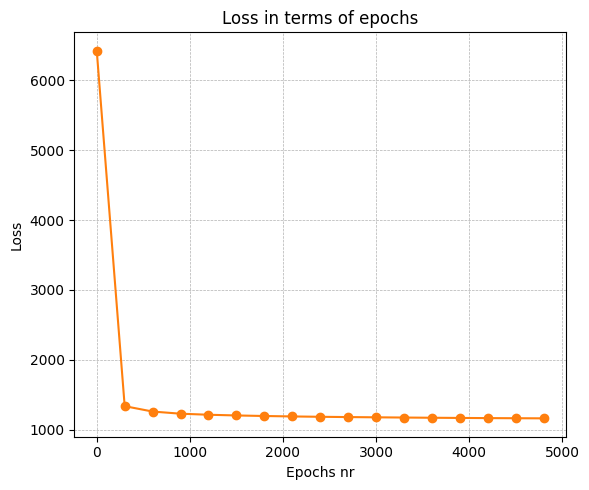
\includegraphics[width=0.45\textwidth]{img/epoch_loss.png}
    \caption{Strata na zbiorze treningowym podczas uczenia}
    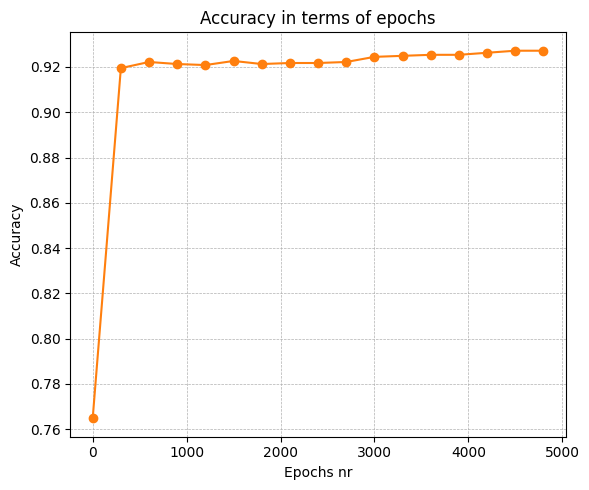
\includegraphics[width=0.45\textwidth]{img/epoch_accuracy.png}
    \caption{Dokładność na zbiorze walidacyjnym podczas uczenia}

\end{figure} \FloatBarrier \\
Zauważyłem, że cokolwiek bym nie robił to strata nigdy \texttt{nie spada} poniżej $2500$. Nie pomagały również algorytmy na bieżąco zarządzające \texttt{learning rate}. Jednak po $1000$ iteracjach zarówno gradient wolno spada, jak i dokładność nie idzie do przodu, więc uznałem $2500$ iteracji za wystarczającą ilość. \smallskip \\
Aby uniknąć przeuczenia, w algorytmie uwzględniłem \texttt{regularyzację L2}, jednak nie dawała ona kompletnie żadnej poprawy. Poniżej przedstawiam rezultaty gdy wyznaczałem współczynnik regularyzacji na zbiorze walidacyjnym. \\
\begin{figure}[h!]
    \centering
    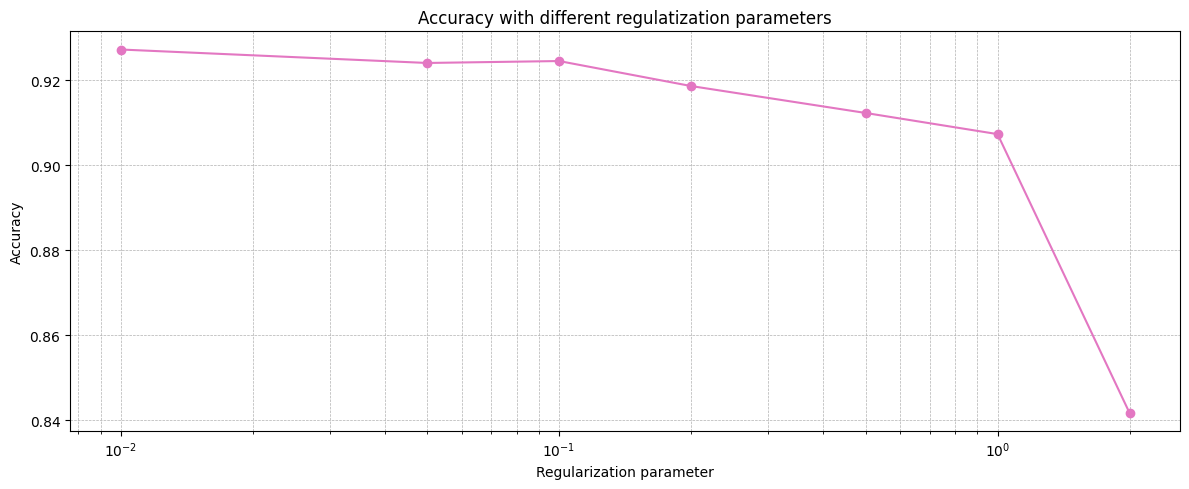
\includegraphics[width=0.60\textwidth]{img/reg_accuracy.png}
    \caption{Dokładnoość na zbiorze walidacyjnym względem współczynnika regularyzacji}
\end{figure} \FloatBarrier \\
Za każdym razem najlepsze wyniki dostawałem bez regularyzacji $L2$, zatem do regresji liniowej zdecydowałem się ją odrzucić.
\section*{SVM - metody jądrowe}
Po napisaniu przeze mnie intefejsu do funkcji $\phi$ przekształcających wektor cech stwierdziłem, że na start warto sprawdzić jaki efekt uzyskam trenując mój model na zbiorze cech będącym wszystkimi kombinacjami pierwotnych cech o stopniu co najwyżej $2$. I owszem, efekt był satysfakcjonujący gdyż uzyskałem w ten sposób dokładność rzędu $93.7\%$. Pojawił się jednak drobny kłopot \textendash\, trenowanie tego modelu zamiast $15$ sekund zajęło mi $15$ minut, a i tak powinienem był go zostawić na jeszcze dłużej bo $1000$ iteracji to było za mało. Zdałem sobie wtedy sprawę że wynik ten był spodziewany \textendash\, zamiast $31$ cech mamy teraz $481$, dodatkowo łączenie tych funkcji też swoje kosztuje więc algorytm spowolnił $60$ krotnie... Stąd podjąłem decyzję, że najlepiej będzie szukać zależości za pomocą funkcji jądrowych. \smallskip \\
Wyniki były niesamowite \textendash\, udało mi się osiągnąć nawet dokładność $96.3\%$. Jednak sam przebieg algorytmu był wymagający obliczeniowo, pojedynczy model potrafił się uczyć po $5$ minut, dlatego zamiast szerszego podsumowania poniżej pokażę wyniki uzyskane przez różne modele. \smallskip \\
Na początku porównajmy jak model z jądrem liniowym wypadnie w kontraście do regresji liniowej. Widzimy że dostajemy zbliżone wyniki, jeśli chodzi o dokładność.
\begin{table}[h!]
\centering
\begin{tabular}{|l|c|}
\hline
\textbf{Metric}     & \textbf{Value} \\
\hline
Accuracy   & 0.9218 \\
Precision  & 0.9186 \\
Sensitivity (Recall) & 0.9432 \\
Specificity & 0.8949 \\
\hline
\end{tabular}
\caption{Wyniki modelu z jądrem liniowym}
\label{tab:metrics}
\end{table}\FloatBarrier
Porównajmy teraz wynik regresji do tego osiągniętego przez jądro kwadratowe. Widzimy że regresja miała jeszcze kilka oczek dokładności do nadgonienia, gdyby się douczyła.
\begin{table}[h!]
\centering
\begin{tabular}{|l|c|}
\hline
\textbf{Metric}     & \textbf{Value} \\
\hline
Accuracy   & 0.9530 \\
Precision  & 0.9498 \\
Sensitivity (Recall) & 0.9667 \\
Specificity & 0.9357 \\
\hline
\end{tabular}
\caption{Wyniki modelu \texttt{poly(2, 1)}}
\label{tab:metrics}
\end{table} \FloatBarrier
Również bardzo ładnie poradził sobie model z jądrem gaussowskim, poniżej wynik jednego z lepszych modeli
\begin{table}[h!]
\centering
\begin{tabular}{|l|c|}
\hline
\textbf{Metric}     & \textbf{Value} \\
\hline
Accuracy   & 0.9625 \\
Precision  & 0.9556 \\
Sensitivity (Recall) & 0.9781 \\
Specificity & 0.9429 \\
\hline
\end{tabular} \FloatBarrier
\caption{Wyniki modelu \texttt{gauusian(0.1)}}
\label{tab:metrics}
\end{table}

Zaskoczeniem dla mnie okazał się gorszy wynik jądra w stylu "wszystko". W retrospekcji mógł on wynikać z przetrenowania tego modelu na danych treningowych.

\begin{table}[h!]
\centering
\begin{tabular}{|l|c|}
\hline
\textbf{Metric}     & \textbf{Value} \\
\hline
Accuracy   & 0.8241 \\
Precision  & 0.8255 \\
Sensitivity (Recall) & 0.8677 \\
Specificity & 0.7694 \\
\hline
\end{tabular}
\caption{Wyniki modelu \texttt{poly(3, 1) + gauusian(0.5) + sigmoid}}
\label{tab:metrics}
\end{table}
Kolejnym algorytmem którym się zająłęm był algorytm \texttt{kNN}
\section*{Algorytm kNN}
Algorytm ten jest przykładem nieliniowego klasyfikatora danych. W przypadku \texttt{kNN} nie ma za bardzo mowy o uczeniu się \textendash\, opiera się on o rozpatrywanie średniej spośród k najbliższych sąsiadów. Zatem wymagającą obliczeniowo częścią było szacowanie nowej danej na podstawie zbioru treningowego. Ku mojemu zaskoczeniu nie poradził sobie on wcale najgorzej. \smallskip \\
Hiperparametr $k$ wyznaczany był w oparciu o zbiór walidacyjny. Rozpatrywałem różne potencjalne $k$, jednak trzymając się ograniczenia względem rozmiaru zbioru treningowego, $k \leq \sqrt{|T|}$. Zatem $k$ szukałem wśród $\{1, 2, 5, 10, 20, 50, 100, 150\}$. \smallskip \\
Nie zdecydowałem się na napisanie żadnych optymalizacji przyspieszających algorytm, gdyż działał satysfakcjonująco szybko i szkoda by było robić to kosztem jego wyników. \smallskip \\
Do porównywania odległości użyłem kilku metryk, między innymi metryki euklidesowej i odległości hamminga. Poniżej znajduje się porównanie wyników moich modeli.


\begin{figure}[h!]
    \centering
    \begin{minipage}[b]{0.48\textwidth}
    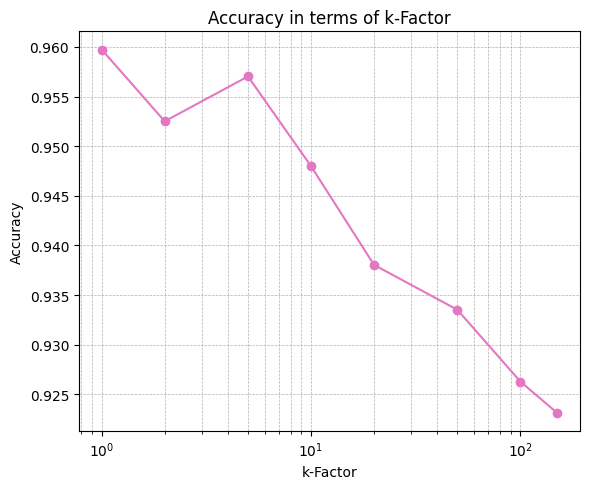
\includegraphics[width=0.9\textwidth]{img/hamming.png}
    \caption{Odległość Hamminga}
    \end{minipage}
     \hspace{0.02\textwidth}
    \begin{minipage}[b]{0.48\textwidth}
    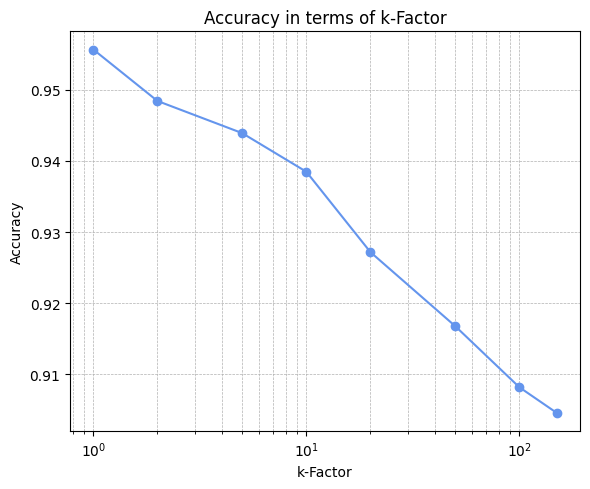
\includegraphics[width=0.9\textwidth]{img/euclidean.png}
    \caption{Odległość Euklidesowa}
    \end{minipage}
\end{figure}
\FloatBarrier

Kolejną rzeczą którą chciałem sprawdzić to jak efektywnie uczy się \texttt{kNN} na frakcjach zbioru treningowego. Poniżej przedstawiam uśrednione wyniki dla najlepszego do tej pory modelu i jego trzech uśrednionych przebiegach dla losowo wybranych podzbiorów.
\begin{figure}[h!]
    \centering
    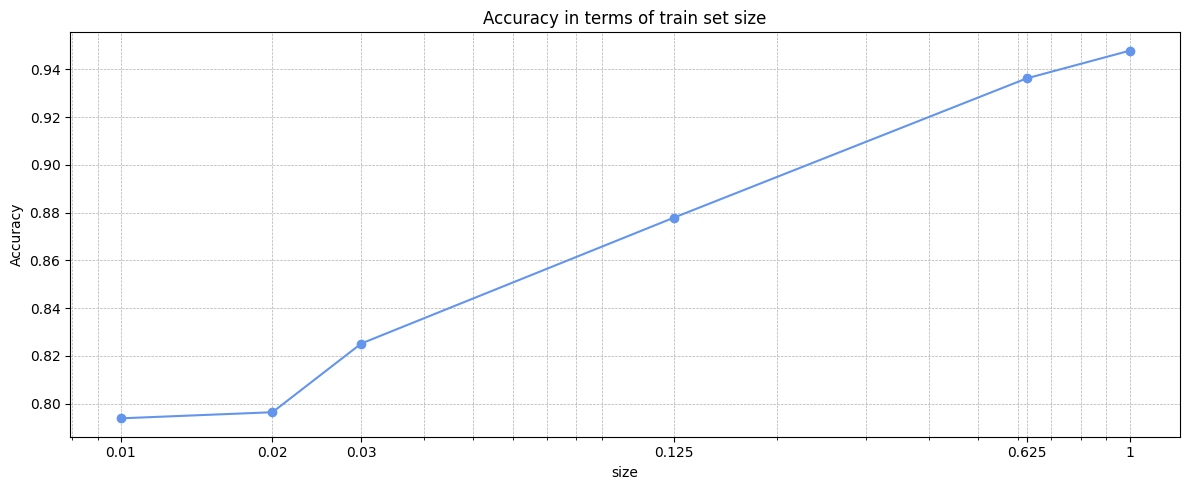
\includegraphics[width=0.60\textwidth]{img/accuracy_size.png}
    \caption{Dokładność dla różnych frakcji zbioru treningowego}
\end{figure} \FloatBarrier \\
Chciałbym zwrócić uwagę na to, że potencjalnie mały procent losowo wybranych danych daje już satysfakcjonujące wyniki. Podsumowując algorytm \texttt{kNN}, zaskakująco $k = 1$ daje w tym przypadku najlepsze rezultaty i to na poziomie $96\%$ dokładności, a wybór metryki nie grał u mnie większej roli.

\section*{Sieci neuronowe}
Ostatnim algorytmem który postanowiłem napisać to sieć neuronowa. Oczywiście nie obyło się bez błędów, najbardziej warte odnotowania jest moje sprawdzenie przez kilka godzin poprawności wzorów gdyż mi błąd nie zbiegał, po czym zdałem sobie sprawę że nie robię wyrazu wolnego. Zaskakująco model potrafił osiągać wtedy nawet $91\%$ dokładności. \smallskip \\
Zdecydowałem się na napisanie modelu sieci w którym poza ustawianiem \texttt{learning rate} i liczby \texttt{epok} będziemy mieli kontrolę nad architekturą ukrytych warstw, zatem możemy podać liczbę warstw sieci i w każdej z nich liczbę neuronów. Jako że to moje pierwsze podejście do sieci neuronowych, zdecydowałem się na początek użyć na każdej z warstw jako funkcji aktywacji funkcji \texttt{sigmoid}.
Moim pierwszym sukcesem było dotrenowanie modelu o kolejnych warstwach rozmiaru $\{31, 200, 200, 2\}$ do $93.5\%$ dokładności. Sprawdźmy teraz jak efektywnie uczą się sieci neuronowe. Poniżej przedstawiam krzywę uczenia dla uproszczonej sieci $\{31, 120, 80, 2\}$. Pierwszy z wykresów odpowiada dokładności na zbiorze walidacyjnym, zaś drugi wartości funkcji straty względem kolejnych epok. Dokładność na zbiorze testowym: $92.7\%$


\begin{figure}[h!]
    \centering
    \begin{minipage}[b]{0.48\textwidth}
    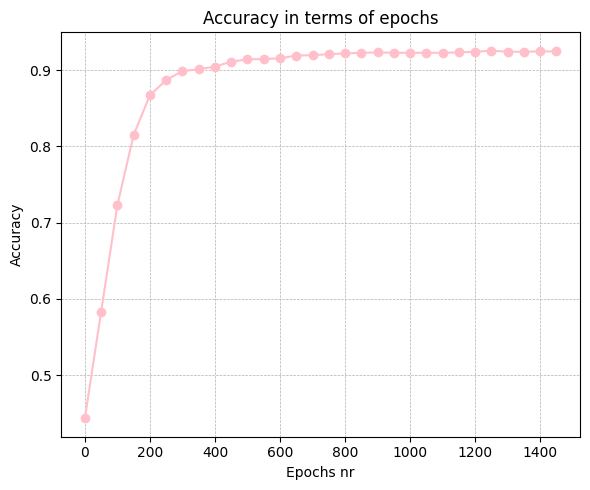
\includegraphics[width=0.9\textwidth]{img/neural_accuracy.png}
    \caption{Dokładność}
    \end{minipage}
     \hspace{0.02\textwidth}
    \begin{minipage}[b]{0.48\textwidth}
    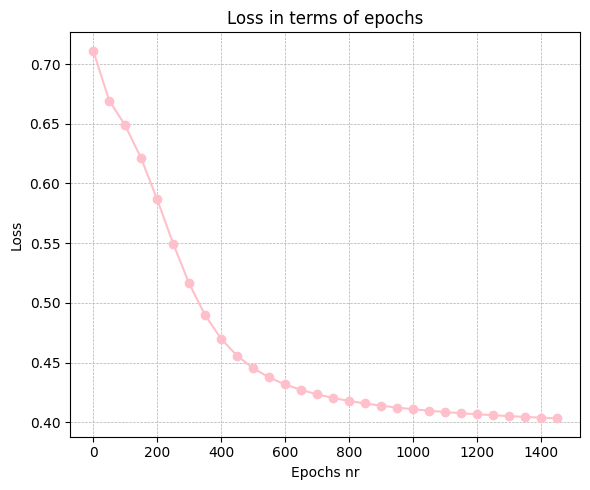
\includegraphics[width=0.9\textwidth]{img/neural_loss.png}
    \caption{Strata}
    \end{minipage}
\end{figure}
\FloatBarrier

Kolejną rzeczą, na którą chciałbym zwrócić uwagę, jest czas uczenia się sieci neuronowej. Zgodnie z wykładem, samo obliczanie danych przez sieć neuronową jest bardzo szybkie, jednak wytrenowanie modeli jest czasochłonne. Pierwszy z omawianych modeli trenowałem $20$ minut przez $2000$ iteracji, zaś drugi \textendash\, ze względu na mniejszy rozmiar warstw i mniejszą liczbę iteracji, $9$ minut. W filmie z kanału \texttt{3blue1brown} mowa jest o praktyczności zastosowania gradientu w wersji \texttt{mini-batch}, jednak nie chciałem tego robić ze względu na to że póki co jakościowo sieć neuronowa wypada najgorzej. \smallskip \\
Zagadkową dla mnie sprawą jest fakt, że nie mogę zbić błędu znacząco poniżej $0.4$. Nie stosuję żadnej regularyzacji, a jednak minimum w które wpadam jest ze stosunkowo dużym błędem. Imponujący jest jednak fakt, że model się uczy szybko i już po $300$ iteracjach jestem w stanie osiągnąć skuteczność na poziomie $90 \% $

\end{document}
